% ==========================================
% SECTION 2: DOMINATOR ANALYSIS
% ==========================================
\section{Dominator Analysis}

L'analisi dei Dominatori è fondamentale per la costruzione della Static Single Assignment (SSA) form e per l'individuazione dei loop naturali nel Control Flow Graph. Un nodo $d$ domina un nodo $n$ se ogni percorso dal nodo di ingresso al nodo $n$ deve passare per $d$.
Spiegazione:
Forward perché i dominatori di un nodo dipendono da chi lo precede, non da chi lo segue
Transfer function: un blocco aggiunge sé stesso all'insieme dei dominatori in ingresso
Boundary: l'Entry domina solo sé stesso all'inizio
Meet = intersezione: un nodo d domina b solo se domina tutti i predecessori di b
Initial = U: iniziamo pessimisticamente (ogni nodo è dominato da tutti), poi l'intersezione raffina
\begin{table}[H]
\centering
\renewcommand{\arraystretch}{1.5}
\begin{tabular}{ll}
\toprule
\textbf{Parameter} & \textbf{Dominator Analysis} \\
\midrule
\textbf{Domain}                    & Sets of nodes (subsets of all basic blocks) \\
\textbf{Direction}                 & Forward: $out[b] = f_b(in[b])$,\quad $in[b] = \wedge out[pred[b]]$ \\
\textbf{Transfer Function}         & $out[b] = \{b\}\cup in[b]$ \\
\textbf{Meet Operation ($\wedge$)} & Intersection ($\cap$) \\
\textbf{Boundary Condition}        & $out[\text{Entry}] = \{\text{Entry}\}$ \\
\textbf{Initial Interior Points}   & $out[B] = \text{U}$ (Universal set) \\
\bottomrule
\end{tabular}
\caption{Dominator Analysis as a Dataflow problem }
\end{table}

Prima aggiungi subito {B} (Gen del nodo stesso)
Intersechi tutti i predecessori (Meet)
Ripeti su tutti i BB finché nessun Dom(B) cambia (convergenza)

Si parte dal massimo possibile (AllNodes)
L'intersezione può solo ridurre gli insiemi, mai aumentarli
Gli insiemi sono finiti -> si converge in al più |AllNodes| iterazioni

\begin{algorithm}[H]
\caption{Dominator Analysis Algorithm}
\begin{algorithmic}[1]
\State $OUT[\text{Entry}] \gets \{\text{Entry}\}$
\For{\textbf{each} basic block $B \neq \text{Entry}$}
    \State $OUT[B] \gets U$
\EndFor
\Statex
\State $changes \gets \text{true}$
\While{$changes$}
    \State $changes \gets \text{false}$
    \For{\textbf{each} basic block $B \neq \text{Entry}$}
        \State $IN[B] \gets \bigcap_{p \in pred(B)} OUT[p]$
        \State $OUT_{new} \gets \{B\} \cup IN[B]$
        \If{$OUT[B] \neq OUT_{new}$}
            \State $OUT[B] \gets OUT_{new}$
            \State $changes \gets \text{true}$
        \EndIf
    \EndFor
\EndWhile
\end{algorithmic}
\end{algorithm}
\vspace{1cm}

\begin{figure}[H]
    \centering
    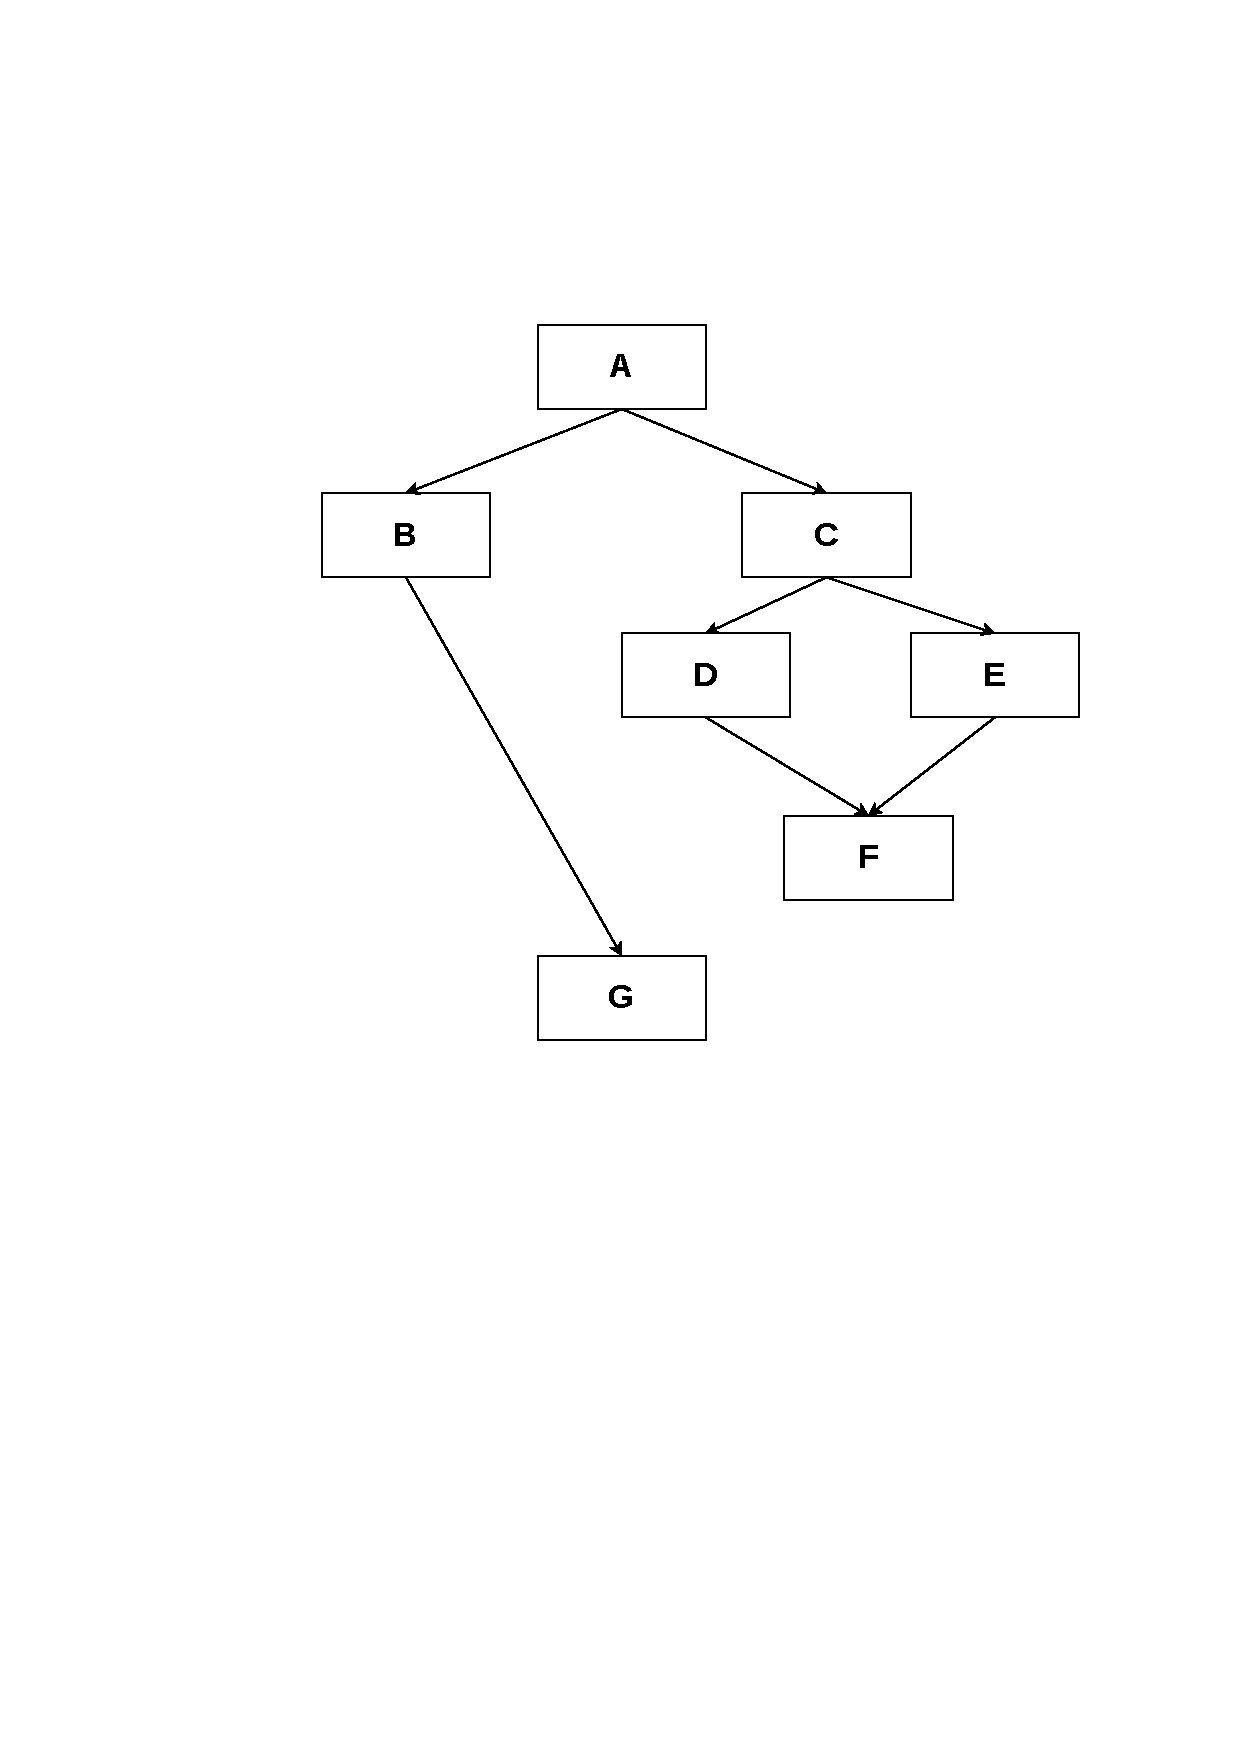
\includegraphics[width=1.0\linewidth]{dominator_analysis_example.pdf}
    \caption{Dominator analysis example CFG}
\end{figure}

Iteraction 1:
Stato iniziale:

OUT[A] = {A} <-  boundary condition
Others = U = {A,B,C,D,E,F,G}

IN[B] = OUT[A] = {A} -> OUT[B] = {A} Union {B} = {A,B}
IN[C] = OUT[A] = {A} -> OUT[C] = {A} Union {C} = {A,C}
IN[D] = OUT[C] = {A,C} -> OUT[D] = {A,C} Union {D} = {A,C,D}
IN[E] = OUT[C] = {A,C} -> OUT[E] = {A,C} Union {E} = {A,C,E}
IN[F] = OUT[D] Intersect OUT[E] = {A,C,D} Intersect {A,C,E} = {A,C} -> OUT[F] = {A,C} Union {F} = {A,C,F}
IN[G] = OUT[B] Intersect OUT[F] = {A,B} Intersect {A,C,F} = {A} -> OUT[G] = {A} Union {G} = {A,G}

Iteraction 2:
Ricalcolo tutto e ottengo gli stessi identici valori -> nessun cambiamento -> fine

\textbf{Stato iniziale:} $OUT[A] = \{A\}$;\quad $OUT[B] = OUT[C] = \cdots = OUT[G] = U$.

\begin{table}[H]
\centering
\renewcommand{\arraystretch}{1.6}
\begin{tabular}{l cc cc}
\toprule
 & \multicolumn{2}{c}{\textbf{Iteration 1}}
 & \multicolumn{2}{c}{\textbf{Iteration 2}} \\
\cmidrule(lr){2-3}\cmidrule(lr){4-5}
\textbf{Block} & \textbf{IN[B]} & \textbf{OUT[B]}
               & \textbf{IN[B]} & \textbf{OUT[B]} \\
\midrule
\textbf{A (Entry)}
    & ---           & $\{A\}$       & ---           & $\{A\}$ \\
\textbf{B}
    & $\{A\}$       & $\{A,B\}$     & $\{A\}$       & $\{A,B\}$ \\
\textbf{C}
    & $\{A\}$       & $\{A,C\}$     & $\{A\}$       & $\{A,C\}$ \\
\textbf{D}
    & $\{A,C\}$     & $\{A,C,D\}$   & $\{A,C\}$     & $\{A,C,D\}$ \\
\textbf{E}
    & $\{A,C\}$     & $\{A,C,E\}$   & $\{A,C\}$     & $\{A,C,E\}$ \\
\textbf{F}
    & $\{A,C\}$     & $\{A,C,F\}$   & $\{A,C\}$     & $\{A,C,F\}$ \\
\textbf{G}
    & $\{A\}$       & $\{A,G\}$     & $\{A\}$       & $\{A,G\}$ \\
\bottomrule
\end{tabular}
\caption{Iteration table for Dominator Analysis on the example CFG.}
\end{table}
